\documentclass[../rapport.tex]{subfiles}
\graphicspath{{\subfix{ressources/photos_diagrammes/app1/gui/}}}


\begin{document}


\subsubsection{Application clients}
Cette section décrit les différents interfaces auxquels les utilisateurs de l'application auront accès pour gérer leurs comptes, portefeuilles et produits financiers.\\

\begin{enumerate}
\item \textbf{LoginScreen} \\
		\begin{figure}[h!]
				\centering 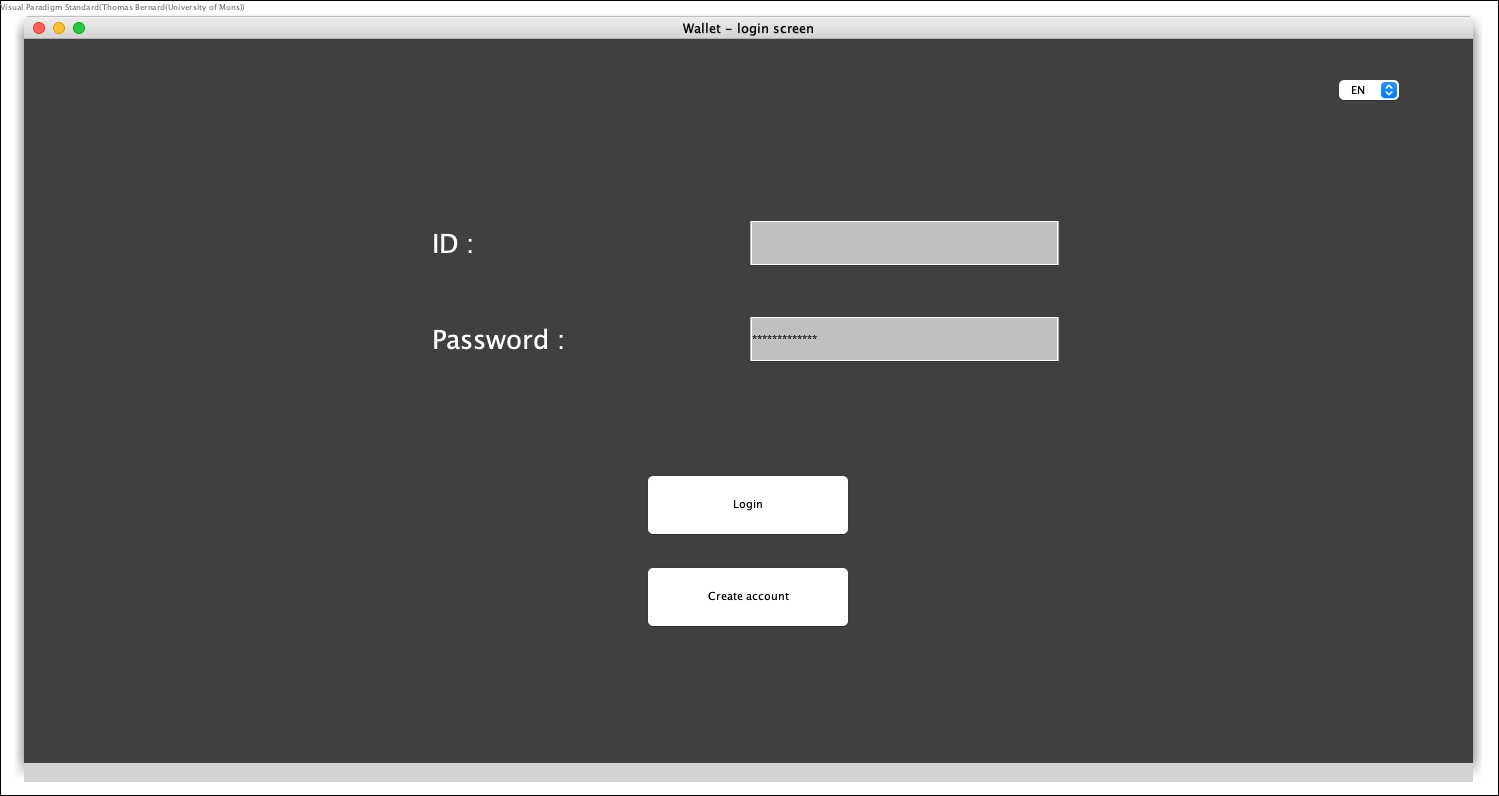
\includegraphics[scale=0.2]{ressources/photos_diagrammes/app1/gui/login.jpg}
				\caption{Login Scene}
		\end{figure}
		\\
L'écran de connexion est la première interface affichée lors du démarrage de l'application.\\
Cette interface permet à l'utilisateur de se connecter via ses identifiants ou d'accéder à l'écran de création de compte.\\
La langue d'affichage peut également être changée directement depuis le coin supérieur droit.

\item \textbf{RegisterScreen} \\
		\begin{figure}[h!]
				\centering 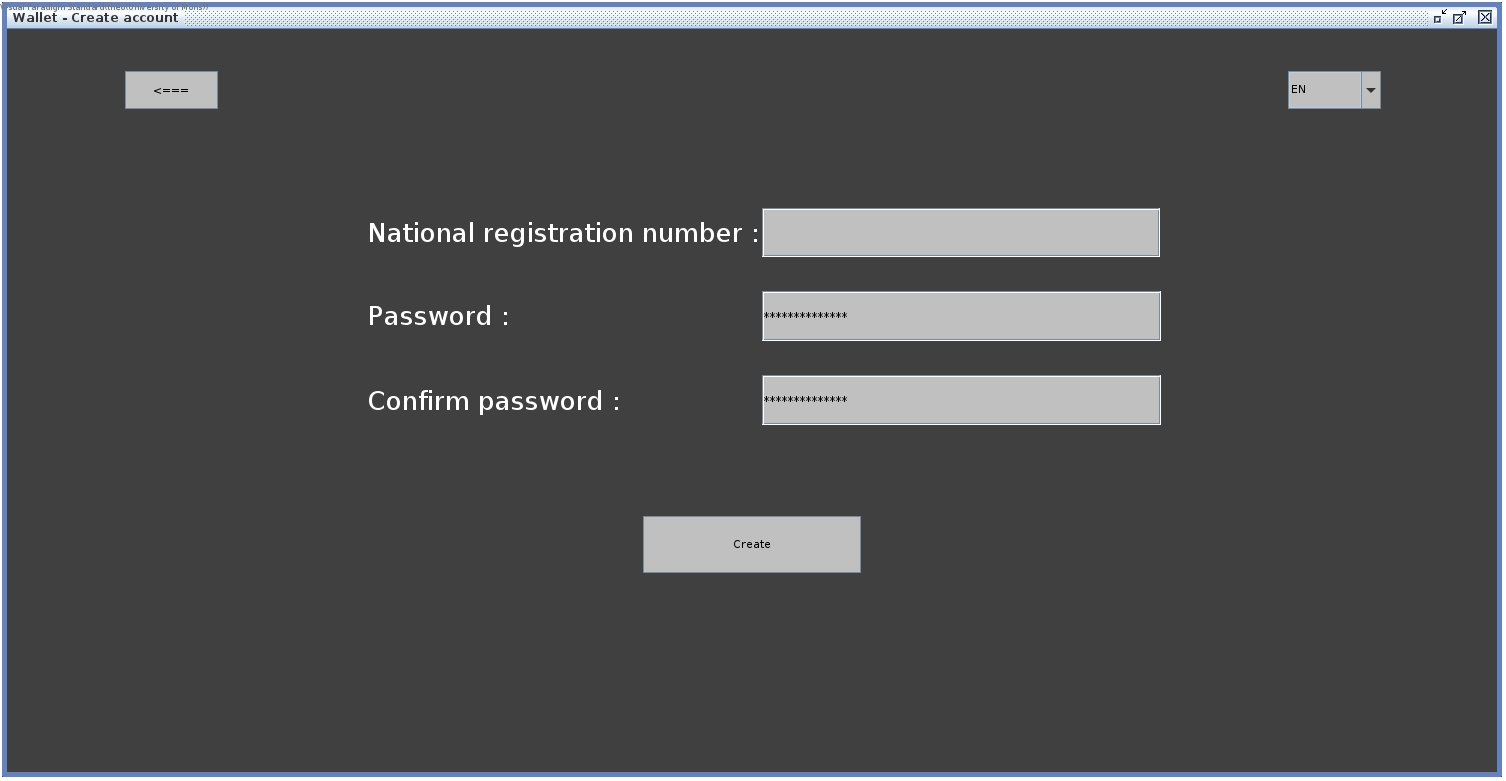
\includegraphics[scale=0.2]{ressources/photos_diagrammes/app1/gui/createAccount.jpg}
				\caption{Login Scene}
		\end{figure}
		\\
Un utilisateur peut s'enregister via cet écran en entrant les données demandées.\\
Le numéro de registre national étant unique, le client ne sera pas en mesure de se créer plusieurs compte sur l'application.\\
Une fois le compte créé, l'utilisateur sera amené à un écran de connexion afin de procéder à l'authentification.

\item \textbf{MainMenuScreen} \\
		\begin{figure}[h!]
				\centering 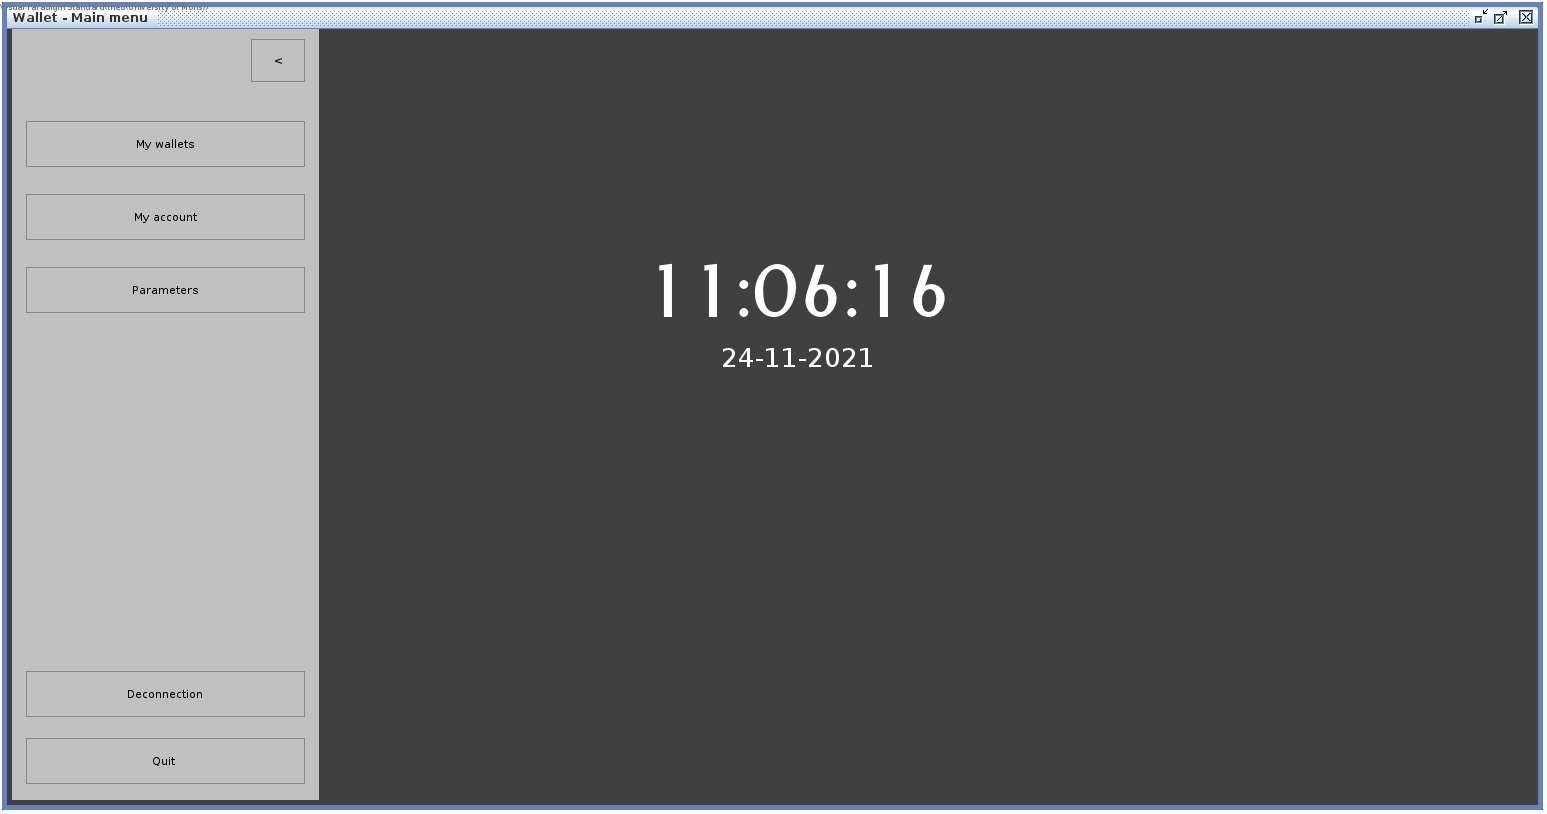
\includegraphics[scale=0.2]{ressources/photos_diagrammes/app1/gui/mainMenu.jpg}
				\caption{Login Scene}
		\end{figure}
		\\
Une fois qu'un utilisateur s'est authentifié via le LoginScreen, le menu principal lui est affiché. Il permet à l'utilisateur d'accéder à toutes ses données via le menu à 
gauche de l'écran. Il contient un bouton ``My wallets'' qui mène l'utilisateur vers l'écran de gestion de ses portefeuilles financiers.\\
Un bouton ``My account'' permet à l'utilisateur d'avoir un écran d'aperçu de ses données. Il pourra aussi changer de mot de passe via cet écran.\\
Le bouton ``Parameters'' mène à l'écran des paramètres de l'app.\\
Le bouton ``Deconnection'' permet de se déconnecter afin de changer d'utilisateur (il mène à l'écran de connexion).\\
Et le bouton ``Quit'' déconnecte l'utilisateur et ferme l'application.
\newpage
\item \textbf{WalletsListScreen} \\
		\begin{figure}[h!]
				\centering 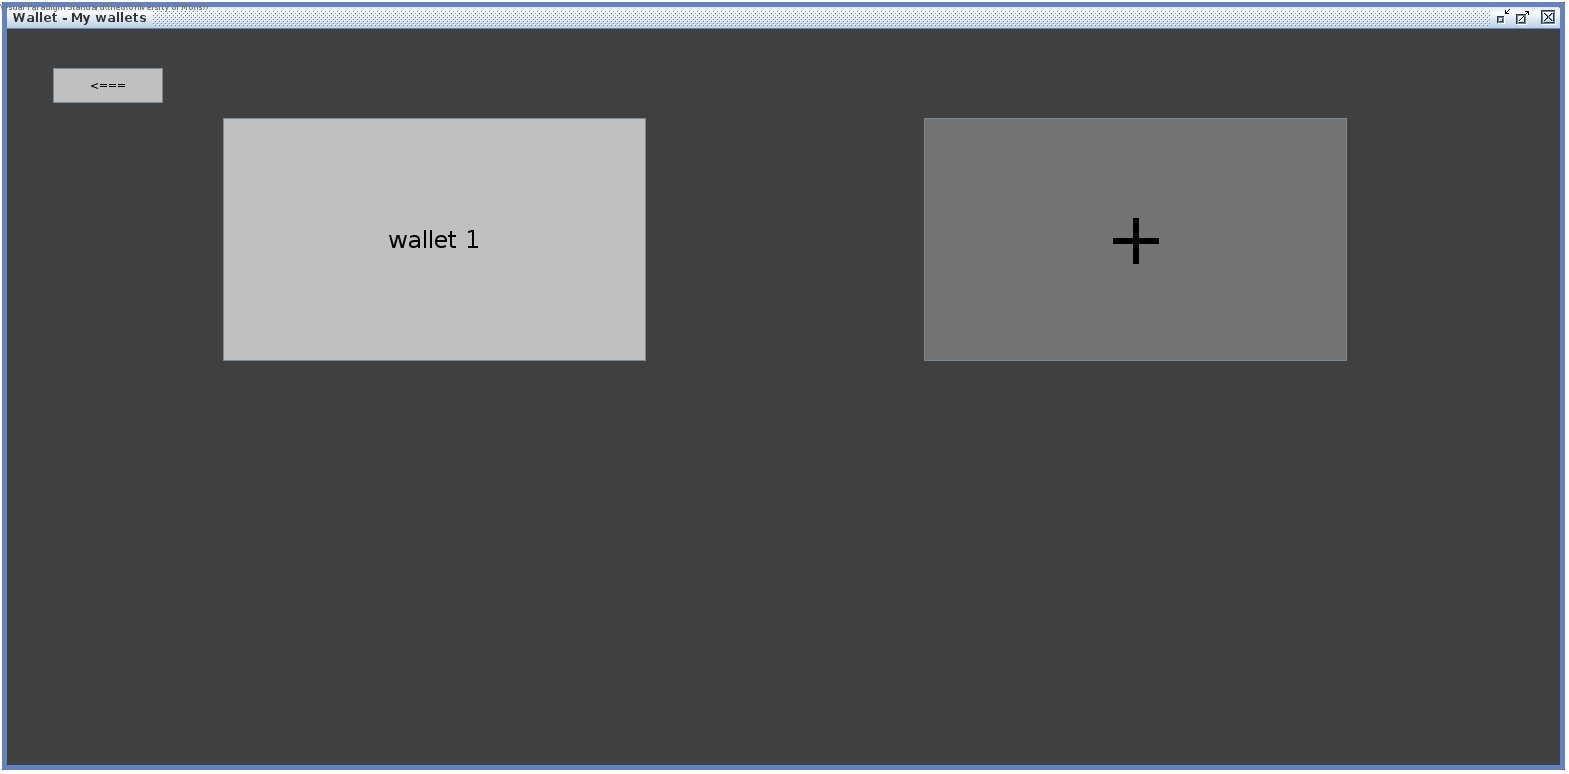
\includegraphics[scale=0.2]{ressources/photos_diagrammes/app1/gui/walletsList.jpg}
				\caption{Wallet List Scene}
		\end{figure}
		\\
Cet écran affiche tous les portefeuilles de l'utilisateur ainsi qu'un bouton permettant d'en ajouter de nouveaux.\\
Les boutons de chaque portefeuille mènent l'utilisateur aux écrans affichant les détails de ceux-ci tandis que le bouton d'ajout de portefeuille envoie sur l'écran de création de portefeuille.\\
L'utilisateur ne pourra créer qu'un portefeuille par institution dont il est client.\\
Un bouton de retour en arrière est aussi présent sur l'écran des portefeuilles afin de permettre à l'utilisateur de retourner au menu princiapl.

\item \textbf{AddWalletScreen} \\
		\begin{figure}[h!]
				\centering 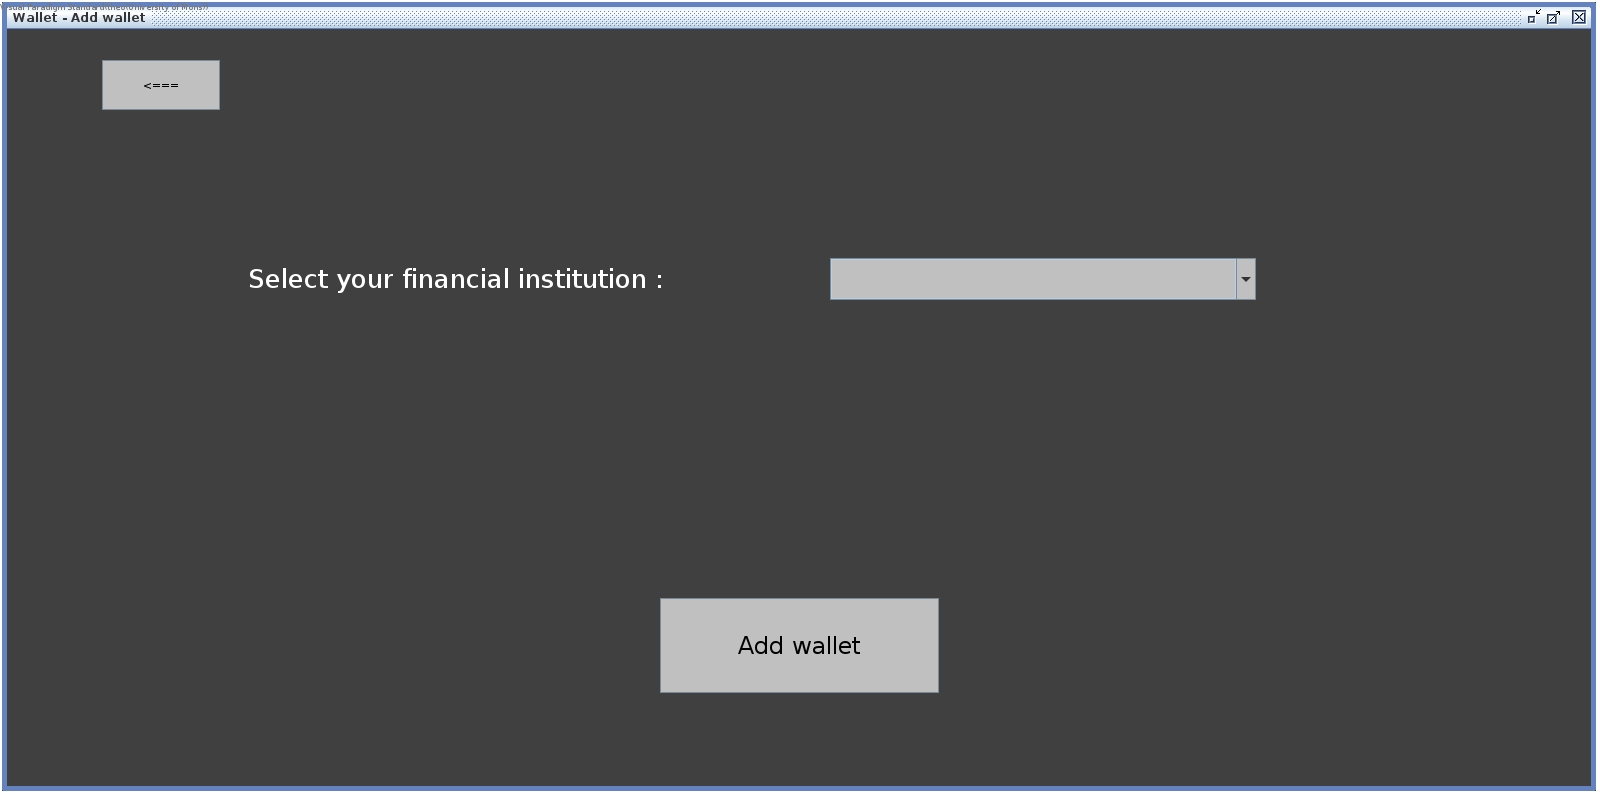
\includegraphics[scale=0.2]{ressources/photos_diagrammes/app1/gui/addWallet.jpg}
				\caption{Scene to add a wallet}
		\end{figure}
		\\
AddWalletScreen propose à l'utilisateur de choisir une institution financière pour laquelle il veut avoir un portefeuille financier visible dans le menu des portefeuilles (WalletsListScreen). Si il est client de cette institution, la demande sera validée et le portefeuille sera accessible.\\
Un bouton retour de en arrière se trouve dans le coin supérieur gauche de l'écran. Ce bouton renvoie vers la liste des portefeuilles de l'utilisateur.
\newpage
\item \textbf{ProductsListScreeen} \\
		\begin{figure}[h!]
				\centering 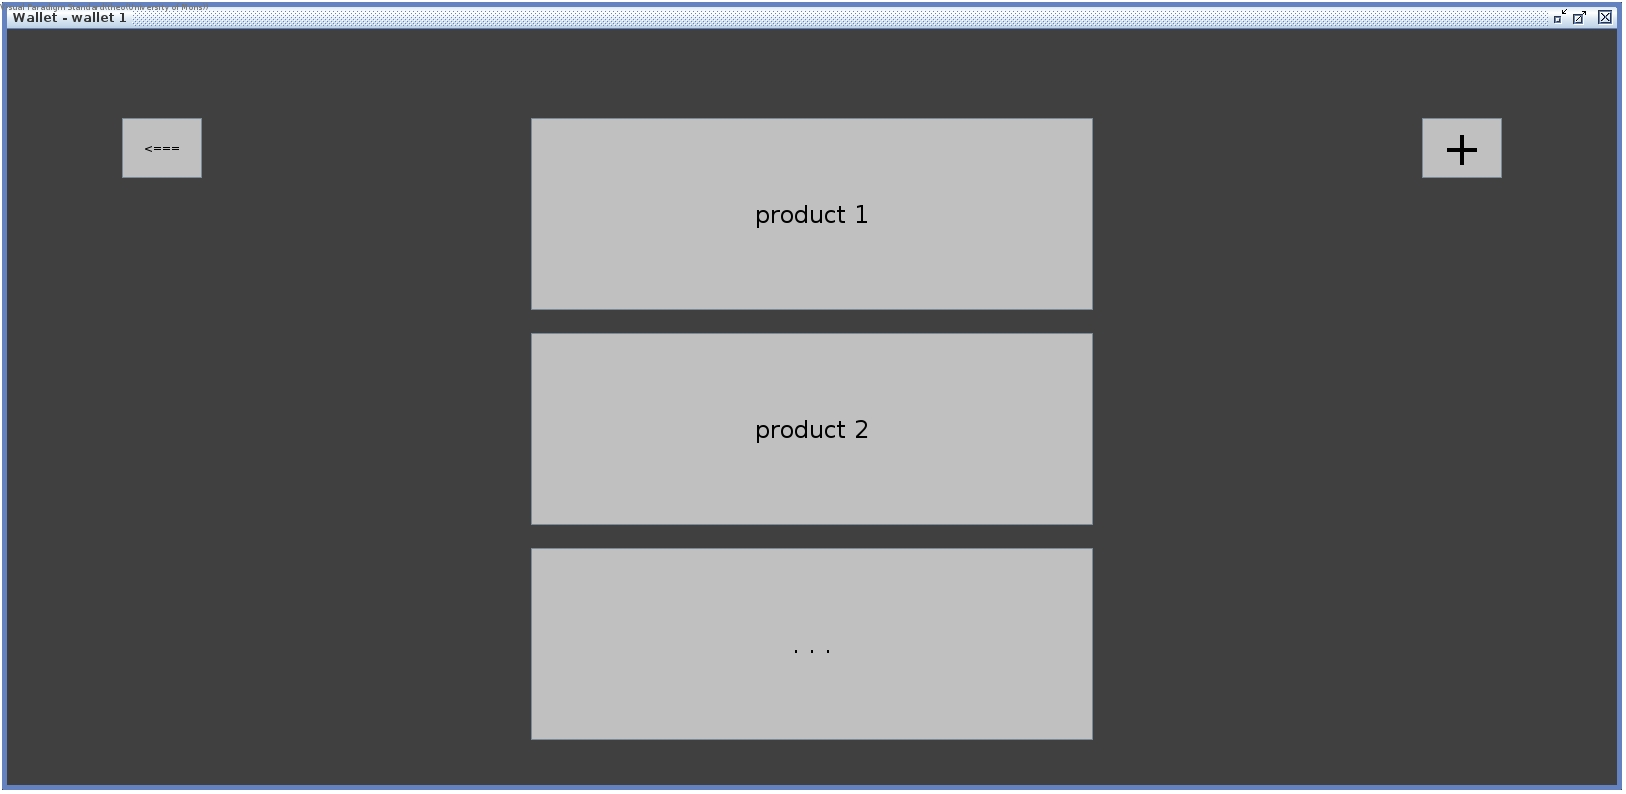
\includegraphics[scale=0.2]{ressources/photos_diagrammes/app1/gui/productsList.jpg}
				\caption{List of the products}
		\end{figure}
		\\
Chaque bouton permet à l'utilisateur de consulter les détails d'un de ses produits financiers.\\
Il peut faire une demande d'ajout de nouveau produit financier. Une fois que celle-ci sera validée par l'institution, le produit créé apparaitra dans la liste du menu précédent.\\
Un bouton de retour en arrière permet de revenir au menu précédent manuellement et donc d'annuler la création du produit financier.
\newpage
\item \textbf{ProductMenuScreen}\\
		\begin{figure}[h!]
				\centering 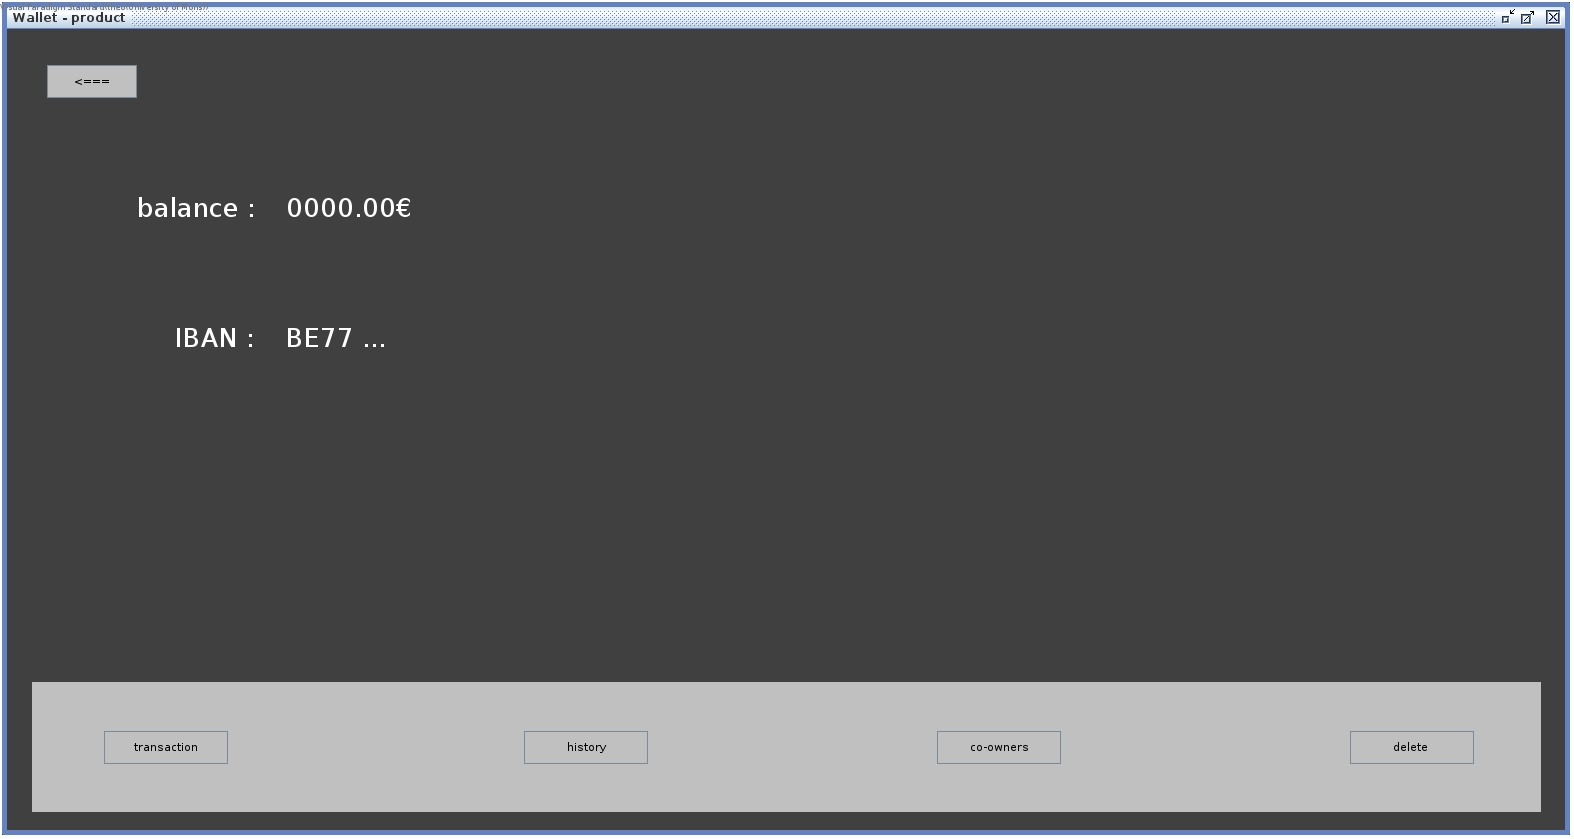
\includegraphics[scale=0.2]{ressources/photos_diagrammes/app1/gui/productMenu.jpg}
				\caption{Product menu}
		\end{figure}
		\\
Cet écran est affiché à l'utilisateur lorsqu'il clique sur un de ses produits financiers. \\
Les informations générales du produit financier (telles que le solde du compte et le numéro de compte) y sont disposées et les boutons du bas de l'écran permettent à l'utilisateur de procéder à différentes opérations sur ce produit financier.\\
Effectuer une transaction se fait via le bouton ``transaction'', consulter l'historique des transactions se fait via le bouton ``history'',
la gesion des co-titulaires se fait via le bouton ``co-owners'' et enfin la suppression du produit se fait via le bouton ``delete''.\\
Le bouton ``delete'' demandera à l'utilisateur de confirmer son action avant de procéder à la désactivation du produit.\\
Un bouton de retour en arrière est également disponible afin de revenir à l'écran du portefeuille dans lequel se trouve le produit financier courrant.

\item \textbf{TransactionScreen}\\
		\begin{figure}[h!]
				\centering 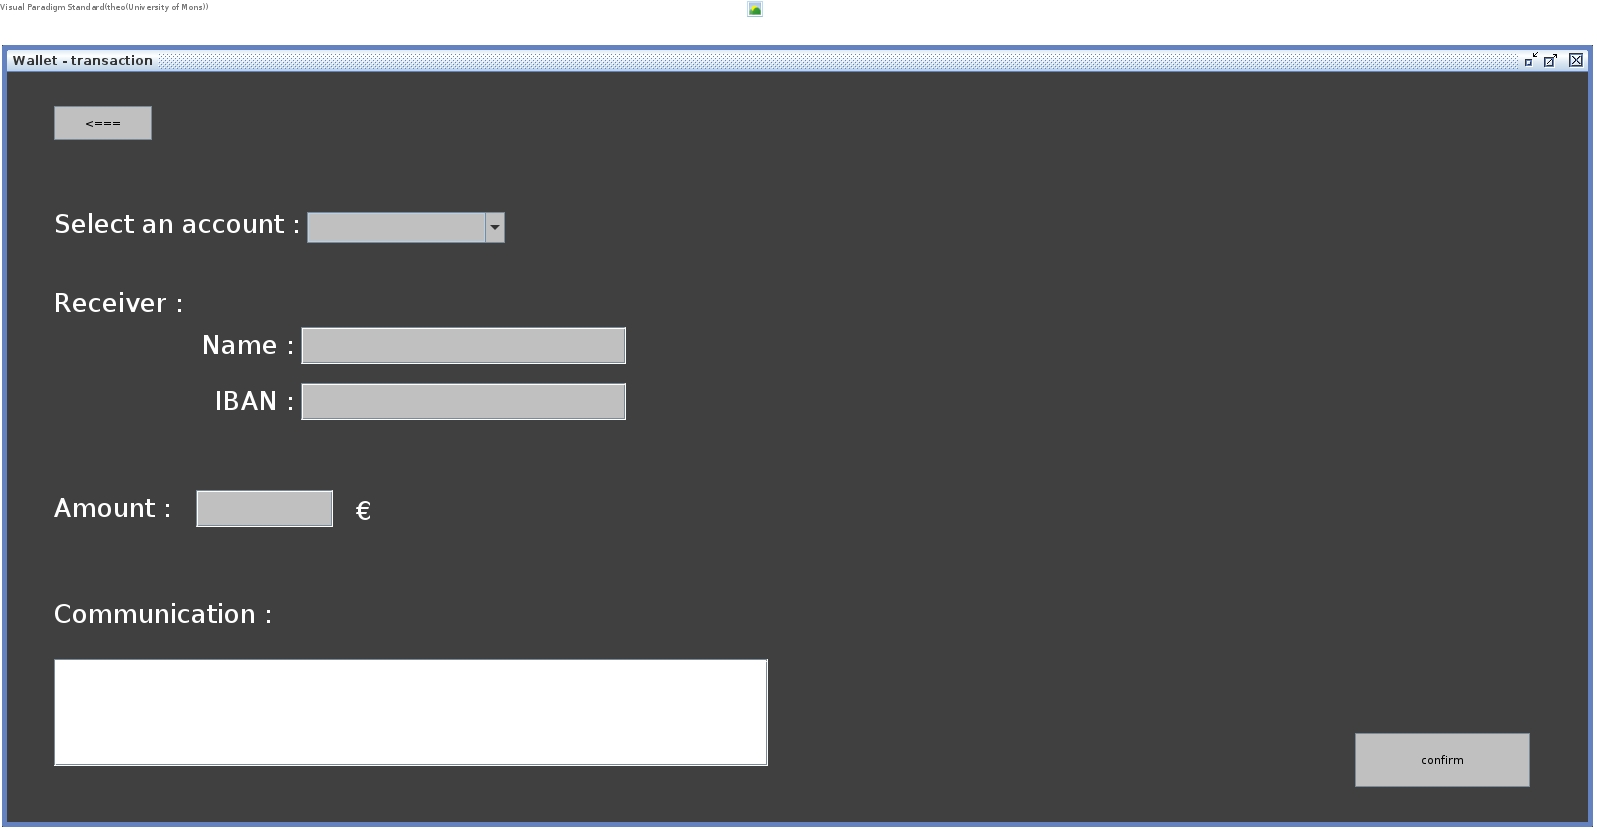
\includegraphics[scale=0.2]{ressources/photos_diagrammes/app1/gui/performTransaction.jpg}
				\caption{Transaction scene}
		\end{figure}
		\\
L'écran de transaction demande plusieurs informations à l'utilisateur afin d'effectuer une transaction d'un compte A à un compte B.\\
Si ce menu a été accéder via le menu d'un produit financier, le compte envoyeur ne peut pas être modifié par l'utilisateur. Sinon, il doit sélectioner un compte parmis tous ceux qu'il possède.\\
Le nom et l'IBAN du receveur doit ensuite être entré dans leurs champs respectifs. Finalement, le montant de la transaction doit être précisé et optionnellement une communication peut être jointe à la transaction.\\
Une fois toutes les données entrées, le bouton ``confirm'' va afficher un résumé de la transaction, l'utilisateur pourra alors décider de confirmer ou annuler la transaction.
Le bouton retour arrière renvoie vers le menu du produit financier et annule la transaction courrante.

\item \textbf{ProductHistoryScreen}\\
		\begin{figure}[h!]
				\centering 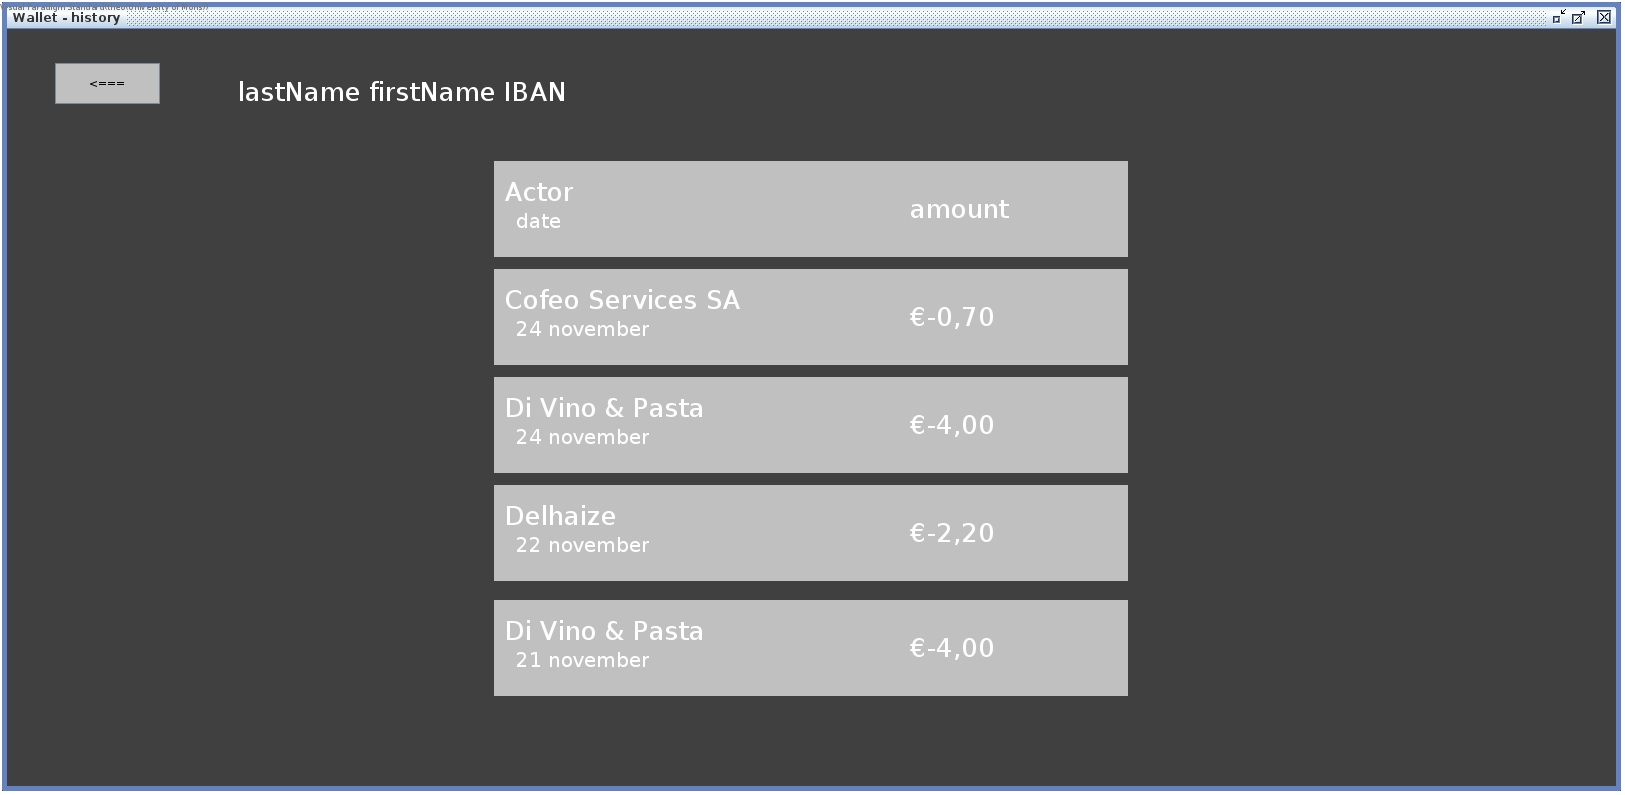
\includegraphics[scale=0.2]{ressources/photos_diagrammes/app1/gui/productHistory.jpg}
				\caption{History of the product}
		\end{figure}
		\\
Cet écran affiche toutes les transactions effectuées depuis et vers le produit courrant.\\
Pour chaque transaction, l'envoyeur ou destinataire est affiché ainsi que la date de l'opération et le montant.\\
Le bouton retour arrière mènera l'utilisateur vers le menu du produit.
\newpage
\item \textbf{OwnersScreen}\\
		\begin{figure}[h!]
				\centering 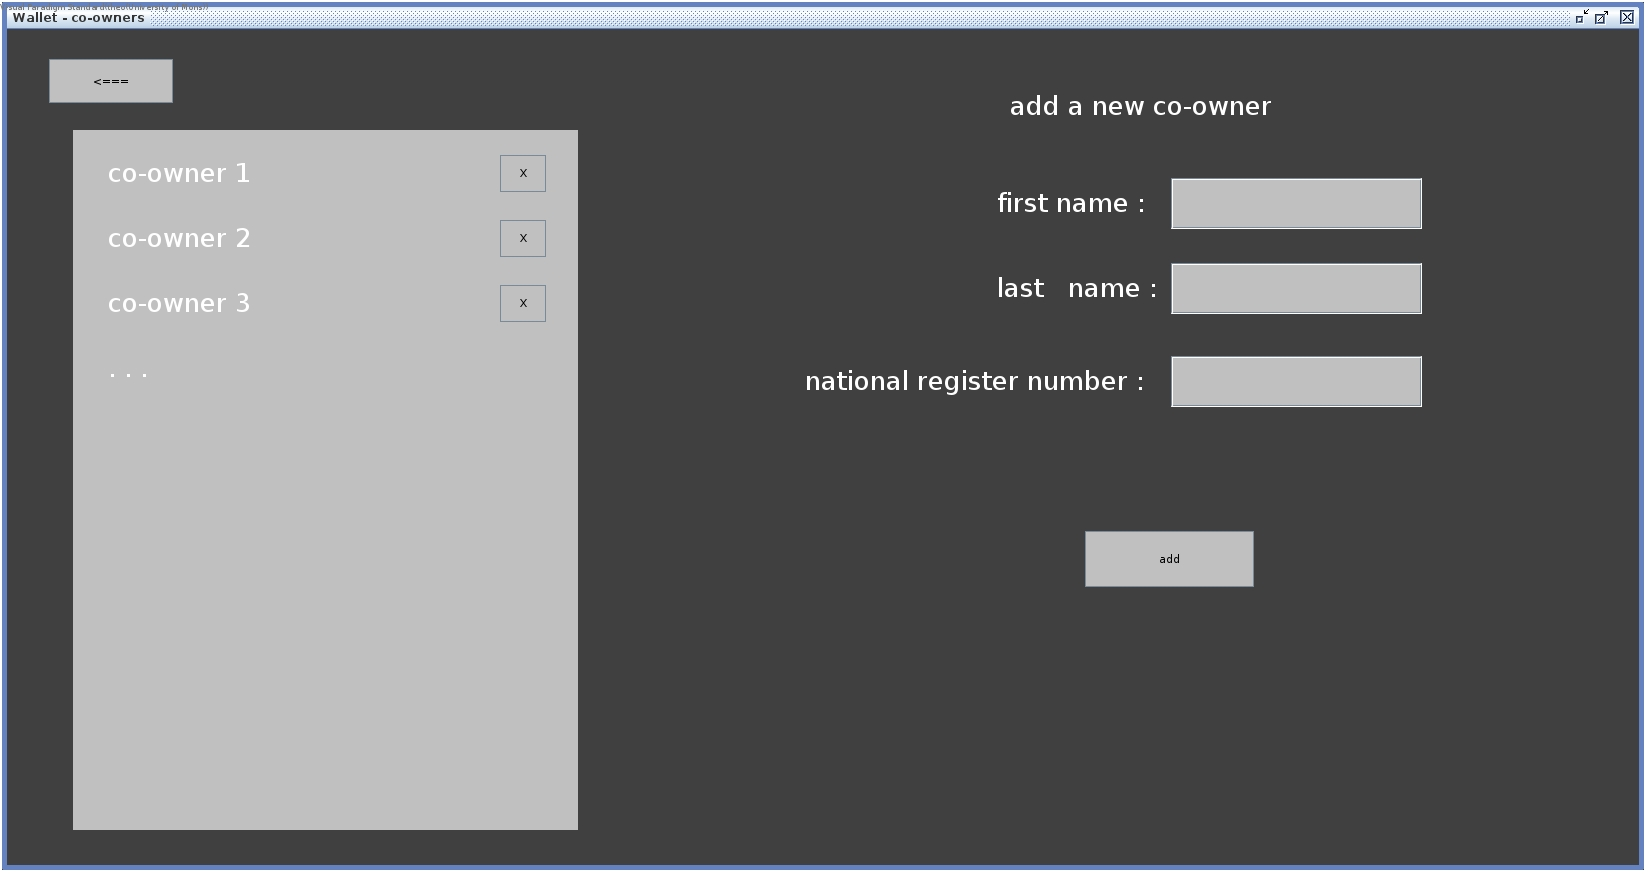
\includegraphics[scale=0.2]{ressources/photos_diagrammes/app1/gui/owners.jpg}
				\caption{Owners scene}
		\end{figure}
		\\
L'écran de gestion des co-titulaires affiche une liste de toutes les personnes partageant le compte.\\
L'utilisateur peut supprimer ou ajouter des co-titulaire via ce menu.\\
Le nom, prénom et numéro de registre nationnal sont nécessaires afin d'ajouter un nouveau co-titulaire.\\
Le bouton de retour arrière renvoie l'utilisateur vers le menu du produit.

\end{enumerate}
\end{document}
